\documentclass[12pt]{article}
%%%%%%%%%%%%%%%%%%%%%%%%%%%%%%%%%%%%%%%%%%%%%%%%%%%%%%%%%%%%%%%%%%%%%%%%%%%%%%%%%%%%%%%%%%%%%%%%%%%%%%%%%%%%%%%%%%%%%%%%%%%%%%%%%%%%%%%%%%%%%%%%%%%%%%%%%%%%%%%%%%%%%%%%%%%%%%%%%%%%%%%%%%%%%%%%%%%%%%%%%%%%%%%%%%%%%%%%%%%%%%%%%%%%%%%%%%%%%%%%%%%%%%%%%%%%
\usepackage{amsfonts}
\usepackage{eurosym}
\usepackage{geometry}
\usepackage{amsmath,amsthm,amssymb}
\usepackage{graphicx}
\usepackage{comment}
%\usepackage[sort,comma]{natbib}
\usepackage[backend=biber, style = apa]{biblatex}
\usepackage{placeins} % to separate sections

\usepackage{adjustbox}
\usepackage{array}
\usepackage{multirow}
\usepackage{graphicx}
\usepackage{subcaption}
\usepackage{pifont}
\usepackage{amssymb}
\usepackage{comment}
\usepackage[utf8]{inputenc}
\usepackage{setspace}
\usepackage[hang, flushmargin, bottom]{footmisc}
\usepackage{footnotebackref}
\usepackage{xcolor}
\usepackage{hyperref}
\usepackage{booktabs}
\usepackage{pifont}
\usepackage{caption}
\usepackage{float}
\usepackage{todonotes}
\setcounter{MaxMatrixCols}{10}
%TCIDATA{OutputFilter=LATEX.DLL}
%TCIDATA{Version=5.50.0.2960}
%TCIDATA{<META NAME="SaveForMode" CONTENT="1">}
%TCIDATA{BibliographyScheme=BibTeX}
%TCIDATA{LastRevised=Sunday, April 28, 2024 18:12:38}
%TCIDATA{<META NAME="GraphicsSave" CONTENT="32">}
%TCIDATA{Language=American English}

%\setlength{\bibsep}{0.3pt}
\setlength{\parskip}{1em}
\setlength{\textfloatsep}{5pt}
\hypersetup{breaklinks=true,hypertexnames=false,colorlinks=true,citecolor = teal}
\captionsetup{font=normalsize}
\newcommand{\cmark}{\ding{51}}
\def\sym#1{\ifmmode^{#1}\else\(^{#1}\)\fi}
\renewcommand{\thetable}{\Roman{table}}
\geometry{verbose,tmargin=.9in,bmargin=1in,lmargin=1in,rmargin=.9in,nomarginpar}
\makeatletter
\DeclareTextSymbolDefault{\textquotedbl}{T1}
\theoremstyle{plain}
\newtheorem{thm}{\protect\theoremname}
\theoremstyle{plain}
\newtheorem{prop}[thm]{\protect\propositionname}
\providecommand{\propositionname}{Proposition}
\providecommand{\theoremname}{Theorem}
\makeatother
\providecommand{\propositionname}{Proposition}
\providecommand{\theoremname}{Theorem}
\newtheorem{ass}[thm]{Assumption}
% \input{tcilatex}
\usepackage{tikz}
\usetikzlibrary{shapes.geometric, arrows, positioning}

\tikzstyle{block} = [rectangle, draw, text width=4cm, align=center, rounded corners, minimum height=1cm]
\tikzstyle{decision} = [rectangle, draw, text width=4cm, align=center, fill=blue!30, minimum height=1cm]
\tikzstyle{arrow} = [->, thick]








\addbibresource{references.bib}
\begin{document}
 
% \title{{\Large Centralized annuities marketplace}}
%\author{Lucas Condeza\thanks{Yale University %\texttt{lucas.schmitz@yale.edu}}} 
%\date{}
%\maketitle
This document provides a comparison between the indicative bidding(IB) setting and the SCOMP process (our setting). We start by outlining the timing of the game in both cases 

\subsection{Indicative bidding}

There are $N$ potential buyers. Initially each bidder observes a private signal/type ($S_i \in \mathbb{R}$) about the value of the asset ($V_i$). 


Before the game starts the seller selects a set of finite messages ($\{0, 1, ..., M\}$). 

The seller also commits to selecting a number of bidders, ($n\leq N$), who send the highest messages to advance to the second stage.


The timing of the game is: 
\begin{enumerate}
    \item Potential bidders simultaneously submit messages, ($m_i$), which are non-binding preliminary bids or indications of interest.  Bidders use a strategy that is weakly increasing in their type ($S_i$).

    \item The $n$ selected bidders incur the entry cost\footnote{For example in takeover auctions, which use an indicative bidding design, the entry cost is due to costly due dilligence. } ($c$), learn their asset value ($V_i$) perfectly, and proceed to the auction.  

    \item Selected bidders, knowing their valuations, bid in a second-price auction, hence they bid their true valuations. 

\end{enumerate}

\subsection{SCOMP}

There are $N$ potential bidders (firms). Initially each bidder observes a private signal type ($S_i \in \mathbb{R}$) about the cost of the servicing the buyer. 

The timing of the game is: 
\begin{enumerate}
    \item Firms make initial bids. 
    \item The buyer observes the bids and requests revised bids from a subset of firms
    \item Firms selected for the revised offer observe the initial offers and realized their revised offers. 
\end{enumerate}

 

\subsection{Relation to our setting}

The similarities between the IB and SCOMP settings are: 
\begin{itemize}
    \item 
In both cases the auction has two stages. 


\end{itemize}

%In the indicative bidding setting (IB) the gain with respect to an unrestricted auction is that reduces the threshold (in terms of type) that makes the bidder indifferent between paying or not paying the entry cost.





But beyond that there are several differences: 

\begin{itemize}
    \item In the IB setting the preliminary bids are not revealed to the other buyers. The learning occurs by paying the entry cost $c$, which in takeover auctions represents the costs the firms have to pay to do due diligence. In the SCOMP setting, it is common that firms observe the first stage bids \footnote{Firms normally request the certificate with the first stage offers to the retiree, from conversations with industry intermediaries, it is common that they comply to the request by sending it.}

    
    \item In an auction with entry costs the seller bears some part of the cost by receiving lower bids, IB increases revenue by decreasing the number of firms paying the entry cost.  In the SCOMP this is not the case since firms do not pay an entry cost. 

    \item In an Indicative bidding auction (IB) the first stage bids are not binding, whereas in our case they are binding. Moreover, initial bids constrain the revised offers since the revise bids can not be lower than the initial ones. 
    
    %\item In IB, the rationale for the seller is that learning  about the value of the good is costly, in the SCOMP it is not.  
\end{itemize}


\vspace{3cm}

 

\newpage

\section{Argument of why is private values}

\textbf{If firms were learnign about the mortality tables then they should update the tables used for future pricing. They do not. Hence, although is common value they behave as if it was private value. }

Firms are indexed by $j$ and individuals by $i$. $x_i$ are individual characteristics observed by all the firms, $r_j$ is the firm specific discount rate and the mortality tables ($f_j(x, r)$). Mortality tables provide an expected cost, given individual characteristics and a discount rate, of selling an annuity that pays one each period\footnote{Actually mortality tables are are a set of survival probabilities. Denote by $Pr(a|x)$ the probability the individual lives at least $a$ additional periods. Using $f_j(x, r)= \sum_{t =0}^\infty Pr(a|x)\frac{1}{(1+r)^t}$, one can construct a mapping from a mortality table to a cost function. }. 

Denote by $f(x, r_j) $ the true cost of firm $j$. We assume that firms do not observe their true cost but receive a noisy signal of it, specifically $f_j(x, r_j) \sim N(f(x_j, r), \sigma_j)$. 

It is obvious from this formulation that the setting is one of common values, since the signal received by the other firms contains information about the hazard rates\footnote{In the language used by \textcite{krishna_auction_2010} the setting is of interdependent values since the costs are not exactly the same. It would be a common value setting if and only if $r_j$ is the same for every single firm. }, which if known affects the posterior of the true cost of the firm. Hence a firm after observing offers could recover $f_{j'}(x, r_{j'})$ and use it to learn about the underlying survival probabilities. 

Even though the setting is one of common values, firms do not use the prices of the other firms to recover the mortality tables those other firms use. From conversations with industry participants, firms have different mortality tables and they are constructed using actuarial calculations, not recovering $Pr_{j'}(a|x)$ from the offers made by other firms. 
One explanation for this industry practice is that mortality tables are highly dimensional, and interest rates move on at least a monthly basis, hence recovering the mortality tables using the observed prices might be more difficult than estimating your own mortality tables from scratch. 

Hence, in practice firms behave as if the setting was one of private values. 



\vspace{2cm}
 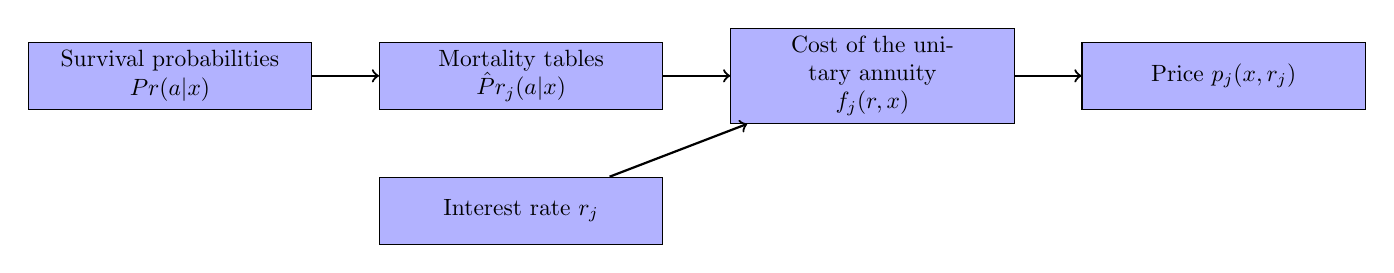
\begin{tikzpicture}[node distance=1cm and 1cm, scale=0.85, every node/.style={transform shape}]

\node[decision] (step1) {Survival probabilities \\ $Pr(a|x)$};
\node[decision, right=of step1] (step2) {Mortality tables \\ $\hat Pr_j(a|x)$};

\node[decision, right=of step2] (step3) {Cost of the unitary annuity \\ $f_j(r,x)$};

\node[decision, right=of step3] (step5) {Price $p_j(x,r_j)$};


\node[decision, below=of step2] (step4) {Interest rate $r_j$};

% **CHANGES MARKED**: Horizontal flow arrows - first row (left to right)
\draw[arrow] (step1) -- (step2);
\draw[arrow] (step2) -- (step3);
\draw[arrow] (step4) -- (step3);
\draw[arrow] (step3) -- (step5);

\end{tikzpicture}
 

\vspace{3cm}


Now consider firms who compete for a sequence of consumers with the same individual characteristics. In what follows, for simplicity we do not use $x$ since all the cosnumers have the same characteristics. 


Moreover the interest rate, which is private information, can change over time $r_{tj} \sim N(r_j, \sigma)$. 


Firms observe the signal of the other firms. 
Then after the first period: 



\vspace{2cm}


There are two cases 
\begin{enumerate}
    \item The firm can recover the mortality tables by observing the signals. In thsi case after many signals there is no further updating. 

    \item The firm can not recover the mortality tables. In this case there is no updating. 
\end{enumerate}


\section{Indicative bidding (Ye)}

One of the results is that \textit{the seller bears the entry cost in equilibrium, and thus the optimal auction is characterized by a finite number of final bidders}, which is not a feature of our setting (page 183). 

In the model each bidder has a private value component before entry, and then they learn from another signal, but there is no learning from the first stage bids (page 183) 


First the individual receives a signal $X_i$ which is a private value component, then bids and the highest $N$ bids are selected. The selected firms pay a cost $c$ and learn $Y_i$. 



There are three cases 
\begin{enumerate}
    \item  pure entry case $Y_i = 0$ which is not our case because there is no learning
    \item Private value updating where the valuation is $X_i  + Y_i$ this is not our case because we want to model a common value auction
    \item Common value updating where the valuation is $X_i + \sum_{j=1}^N Y_j/N$ which is the one we are interested in. Particularly the case where $Y_j = X_j$
\end{enumerate}

The only revelation of information between the first and second round of bidding is the highest non-selected bid. 



\printbibliography
 
\end{document}
